%%
%% Automatically generated file from DocOnce source
%% (https://github.com/hplgit/doconce/)
%%

% #define PREAMBLE

% #ifdef PREAMBLE
%-------------------- begin preamble ----------------------

\documentclass[%
oneside,                 % oneside: electronic viewing, twoside: printing
final,                   % draft: marks overfull hboxes, figures with paths
10pt]{article}

\listfiles               %  print all files needed to compile this document

\usepackage{relsize,makeidx,color,setspace,amsmath,amsfonts,amssymb}
\usepackage[table]{xcolor}
\usepackage{bm,ltablex,microtype}

\usepackage[pdftex]{graphicx}

% Packages for typesetting blocks of computer code
\usepackage{fancyvrb,framed,moreverb}

% Define colors
\definecolor{orange}{cmyk}{0,0.4,0.8,0.2}
\definecolor{tucorange}{rgb}{1.0,0.64,0}
\definecolor{darkorange}{rgb}{.71,0.21,0.01}
\definecolor{darkgreen}{rgb}{.12,.54,.11}
\definecolor{myteal}{rgb}{.26, .44, .56}
\definecolor{gray}{gray}{0.45}
\definecolor{mediumgray}{gray}{.8}
\definecolor{lightgray}{gray}{.95}
\definecolor{brown}{rgb}{0.54,0.27,0.07}
\definecolor{purple}{rgb}{0.5,0.0,0.5}
\definecolor{darkgray}{gray}{0.25}
\definecolor{darkblue}{rgb}{0,0.08,0.45}
\definecolor{darkblue2}{rgb}{0,0,0.8}
\definecolor{lightred}{rgb}{1.0,0.39,0.28}
\definecolor{lightgreen}{rgb}{0.48,0.99,0.0}
\definecolor{lightblue}{rgb}{0.53,0.81,0.92}
\definecolor{lightblue2}{rgb}{0.3,0.3,1.0}
\definecolor{lightpurple}{rgb}{0.87,0.63,0.87}
\definecolor{lightcyan}{rgb}{0.5,1.0,0.83}

\colorlet{comment_green}{green!50!black}
\colorlet{string_red}{red!60!black}
\colorlet{keyword_pink}{magenta!70!black}
\colorlet{indendifier_green}{green!70!white}

% Backgrounds for code
\definecolor{cbg_gray}{rgb}{.95, .95, .95}
\definecolor{bar_gray}{rgb}{.92, .92, .92}

\definecolor{cbg_yellowgray}{rgb}{.95, .95, .85}
\definecolor{bar_yellowgray}{rgb}{.95, .95, .65}

\colorlet{cbg_yellow2}{yellow!10}
\colorlet{bar_yellow2}{yellow!20}

\definecolor{cbg_yellow1}{rgb}{.98, .98, 0.8}
\definecolor{bar_yellow1}{rgb}{.98, .98, 0.4}

\definecolor{cbg_red1}{rgb}{1, 0.85, 0.85}
\definecolor{bar_red1}{rgb}{1, 0.75, 0.85}

\definecolor{cbg_blue1}{rgb}{0.87843, 0.95686, 1.0}
\definecolor{bar_blue1}{rgb}{0.7,     0.95686, 1}

\usepackage{listingsutf8}

% Common lstlisting parameters

\usepackage{calc}
\newlength{\lstboxwidth}  % width of lst box
\newlength{\framethickness}
\setlength{\framethickness}{0.5mm}
% for frame=trbl and a framerule that has significant size, set
% xleftmargin=5mm and xrightmargin=5mm.

\lstset{
  basicstyle=\small \ttfamily,
  breaklines=false,          % break/wrap lines
  breakatwhitespace=true,    % let linebreaks happen at whitespace
  breakindent=40pt,
  tab=,
  tabsize=4,                 % tab means 4 spaces
  %belowskip=\smallskipamount,  % space between code and text below
  xleftmargin=2mm,           % indentation of code frame
  xrightmargin=0mm,
  framexleftmargin=2mm,      % add frame space to the left of the code box
  %numbers=left,             % put line numbers on the left
  %stepnumber=2,             % stepnumber=1 numbers each line, =n every n lines
  framerule=\framethickness, % thickness of frame
  aboveskip=2ex,             % vertical space above code frame
  showstringspaces=false,    % show spaces in strings with an underscore
  showspaces=false,          % show spaces with an underscore
  showtabs=false,
  keepspaces=true,
  columns=fullflexible,      % tighter character kerning, like verb
  escapeinside={(*@}{@*)},   % (*@ \pause @*) in slides and math in code blocks
  extendedchars=\true,       % allows non-ascii chars, does not work with utf-8
}

% Internally defined styles for lstlisting

% Use this one without additional background color
\lstdefinestyle{blue1}{              % blue1 background for code snippets
backgroundcolor=\color{cbg_blue1},
}

% Use this one without additional background color
% (same as blue1, but with bar_blue1 frame)
\lstdefinestyle{blue1bar}{           % blue1 background for complete programs
backgroundcolor=\color{cbg_blue1},
frame=tb,                            % include frame
rulecolor=\color{bar_blue1},         % frame color
}

% Use this one without additional background color
\lstdefinestyle{gray}{
backgroundcolor=\color{cbg_gray},
%frame=tb,                            % include frame
%framerule=0.4pt                      % thickness of frame
rulecolor=\color{black!40},           % frame color
}

\lstdefinestyle{simple}{
commentstyle={},
}

% end of custom lstdefinestyles

\usepackage[T1]{fontenc}
%\usepackage[latin1]{inputenc}
\usepackage{ucs}
\usepackage[utf8x]{inputenc}

\usepackage{lmodern}         % Latin Modern fonts derived from Computer Modern

% Hyperlinks in PDF:
\definecolor{linkcolor}{rgb}{0,0,0.4}
\usepackage{hyperref}
\hypersetup{
    breaklinks=true,
    colorlinks=true,
    linkcolor=linkcolor,
    urlcolor=linkcolor,
    citecolor=black,
    filecolor=black,
    %filecolor=blue,
    pdfmenubar=true,
    pdftoolbar=true,
    bookmarksdepth=3   % Uncomment (and tweak) for PDF bookmarks with more levels than the TOC
    }
%\hyperbaseurl{}   % hyperlinks are relative to this root

\setcounter{tocdepth}{2}  % levels in table of contents

%\VerbatimFootnotes must come after hyperref and footmisc packages
\VerbatimFootnotes

% Tricks for having figures close to where they are defined:
% 1. define less restrictive rules for where to put figures
\setcounter{topnumber}{2}
\setcounter{bottomnumber}{2}
\setcounter{totalnumber}{4}
\renewcommand{\topfraction}{0.95}
\renewcommand{\bottomfraction}{0.95}
\renewcommand{\textfraction}{0}
\renewcommand{\floatpagefraction}{0.75}
% floatpagefraction must always be less than topfraction!
% 2. ensure all figures are flushed before next section
\usepackage[section]{placeins}
% 3. enable begin{figure}[H] (often leads to ugly pagebreaks)
%\usepackage{float}\restylefloat{figure}

% --- fancyhdr package for fancy headers ---
\usepackage{fancyhdr}
\fancyhf{} % sets both header and footer to nothing
\renewcommand{\headrulewidth}{0pt}
\fancyfoot[LE,RO]{\thepage}
% Ensure copyright on titlepage (article style) and chapter pages (book style)
\fancypagestyle{plain}{
  \fancyhf{}
  \fancyfoot[C]{{\footnotesize \copyright\ 2018-2019, Christian Forssén. Released under CC Attribution-NonCommercial 4.0 license}}
%  \renewcommand{\footrulewidth}{0mm}
  \renewcommand{\headrulewidth}{0mm}
}
% Ensure copyright on titlepages with \thispagestyle{empty}
\fancypagestyle{empty}{
  \fancyhf{}
  \fancyfoot[C]{{\footnotesize \copyright\ 2018-2019, Christian Forssén. Released under CC Attribution-NonCommercial 4.0 license}}
  \renewcommand{\footrulewidth}{0mm}
  \renewcommand{\headrulewidth}{0mm}
}

\pagestyle{fancy}


\usepackage[framemethod=TikZ]{mdframed}

% --- begin definitions of admonition environments ---

% Admonition style "mdfbox" is an oval colored box based on mdframed
% "notice" admon
\definecolor{mdfbox_notice_background}{rgb}{1,1,1}
\newmdenv[
  skipabove=15pt,
  skipbelow=15pt,
  outerlinewidth=0,
  backgroundcolor=mdfbox_notice_background,
  linecolor=black,
  linewidth=2pt,       % frame thickness
  frametitlebackgroundcolor=mdfbox_notice_background,
  frametitlerule=true,
  frametitlefont=\normalfont\bfseries,
  shadow=false,        % frame shadow?
  shadowsize=11pt,
  leftmargin=0,
  rightmargin=0,
  roundcorner=5,
  needspace=0pt,
]{notice_mdfboxmdframed}

\newenvironment{notice_mdfboxadmon}[1][]{
\begin{notice_mdfboxmdframed}[frametitle=#1]
}
{
\end{notice_mdfboxmdframed}
}

% Admonition style "mdfbox" is an oval colored box based on mdframed
% "summary" admon
\definecolor{mdfbox_summary_background}{rgb}{1,1,1}
\newmdenv[
  skipabove=15pt,
  skipbelow=15pt,
  outerlinewidth=0,
  backgroundcolor=mdfbox_summary_background,
  linecolor=black,
  linewidth=2pt,       % frame thickness
  frametitlebackgroundcolor=mdfbox_summary_background,
  frametitlerule=true,
  frametitlefont=\normalfont\bfseries,
  shadow=false,        % frame shadow?
  shadowsize=11pt,
  leftmargin=0,
  rightmargin=0,
  roundcorner=5,
  needspace=0pt,
]{summary_mdfboxmdframed}

\newenvironment{summary_mdfboxadmon}[1][]{
\begin{summary_mdfboxmdframed}[frametitle=#1]
}
{
\end{summary_mdfboxmdframed}
}

% Admonition style "mdfbox" is an oval colored box based on mdframed
% "warning" admon
\definecolor{mdfbox_warning_background}{rgb}{1,1,1}
\newmdenv[
  skipabove=15pt,
  skipbelow=15pt,
  outerlinewidth=0,
  backgroundcolor=mdfbox_warning_background,
  linecolor=black,
  linewidth=2pt,       % frame thickness
  frametitlebackgroundcolor=mdfbox_warning_background,
  frametitlerule=true,
  frametitlefont=\normalfont\bfseries,
  shadow=false,        % frame shadow?
  shadowsize=11pt,
  leftmargin=0,
  rightmargin=0,
  roundcorner=5,
  needspace=0pt,
]{warning_mdfboxmdframed}

\newenvironment{warning_mdfboxadmon}[1][]{
\begin{warning_mdfboxmdframed}[frametitle=#1]
}
{
\end{warning_mdfboxmdframed}
}

% Admonition style "mdfbox" is an oval colored box based on mdframed
% "question" admon
\definecolor{mdfbox_question_background}{rgb}{1,1,1}
\newmdenv[
  skipabove=15pt,
  skipbelow=15pt,
  outerlinewidth=0,
  backgroundcolor=mdfbox_question_background,
  linecolor=black,
  linewidth=2pt,       % frame thickness
  frametitlebackgroundcolor=mdfbox_question_background,
  frametitlerule=true,
  frametitlefont=\normalfont\bfseries,
  shadow=false,        % frame shadow?
  shadowsize=11pt,
  leftmargin=0,
  rightmargin=0,
  roundcorner=5,
  needspace=0pt,
]{question_mdfboxmdframed}

\newenvironment{question_mdfboxadmon}[1][]{
\begin{question_mdfboxmdframed}[frametitle=#1]
}
{
\end{question_mdfboxmdframed}
}

% Admonition style "mdfbox" is an oval colored box based on mdframed
% "block" admon
\definecolor{mdfbox_block_background}{rgb}{1,1,1}
\newmdenv[
  skipabove=15pt,
  skipbelow=15pt,
  outerlinewidth=0,
  backgroundcolor=mdfbox_block_background,
  linecolor=black,
  linewidth=2pt,       % frame thickness
  frametitlebackgroundcolor=mdfbox_block_background,
  frametitlerule=true,
  frametitlefont=\normalfont\bfseries,
  shadow=false,        % frame shadow?
  shadowsize=11pt,
  leftmargin=0,
  rightmargin=0,
  roundcorner=5,
  needspace=0pt,
]{block_mdfboxmdframed}

\newenvironment{block_mdfboxadmon}[1][]{
\begin{block_mdfboxmdframed}[frametitle=#1]
}
{
\end{block_mdfboxmdframed}
}

% --- end of definitions of admonition environments ---

% prevent orhpans and widows
\clubpenalty = 10000
\widowpenalty = 10000

% --- end of standard preamble for documents ---


\usepackage[swedish]{babel}

\raggedbottom
\makeindex
\usepackage[totoc]{idxlayout}   % for index in the toc
\usepackage[nottoc]{tocbibind}  % for references/bibliography in the toc

%-------------------- end preamble ----------------------

\begin{document}

% matching end for #ifdef PREAMBLE
% #endif

\newcommand{\exercisesection}[1]{\subsection*{#1}}

\input{newcommands_keep}

% ------------------- main content ----------------------



% ----------------- title -------------------------

\thispagestyle{empty}

\begin{center}
{\LARGE\bf
\begin{spacing}{1.25}
Learning from data: Basics of Bayesian Statistics
\end{spacing}
}
\end{center}

% ----------------- author(s) -------------------------

\begin{center}
{\bf Christian Forssén}
\end{center}

    \begin{center}
% List of all institutions:
\centerline{{\small Department of Physics, Chalmers University of Technology, Sweden}}
\end{center}
    
% ----------------- end author(s) -------------------------

% --- begin date ---
\begin{center}
Sep 12, 2019
\end{center}
% --- end date ---

\vspace{1cm}


% !split
\section{How do you feel about statistics?}
% !bpop

\begin{block_mdfboxadmon}[]
Disraeli (attr.): 

\begin{quote}
“There are three kinds of lies: lies, damned lies, and statistics.”
\end{quote}
\end{block_mdfboxadmon} % title: 


% !epop

% !bpop

\begin{block_mdfboxadmon}[]
Rutherford:

\begin{quote}
“If your result needs a statistician then you should design a better experiment.”
\end{quote}
\end{block_mdfboxadmon} % title: 


% !epop

% !bpop

\begin{block_mdfboxadmon}[]
Laplace:

\begin{quote}
“La théorie des probabilités n'est que le bon sens réduit au calcul”
\end{quote}
\end{block_mdfboxadmon} % title: 


% !epop

% !bpop
Bayesian Methods: rules of statistical inference are an application of the laws of probability
% !epop


% !split
\subsection{Inference}

\begin{block_mdfboxadmon}[]
\begin{itemize}
 \item Deductive inference. Cause $\to$ Effect. 

 \item Inference to best explanation. Effect $\to$ Cause. 

 \item Scientists need a way to:
\begin{itemize}

    \item Quantify the strength of inductive inferences;

    \item Update that quantification as they acquire new data.
\end{itemize}

\noindent
\end{itemize}

\noindent
\end{block_mdfboxadmon} % title: 



% !split
\subsection{Some history}
Adapted from D.S. Sivia\footnote{Sivia, Devinderjit, and John Skilling. Data Analysis : A Bayesian Tutorial, OUP Oxford, 2006}:




\begin{quote}
Although the frequency definition appears to be more objective, its range of validity is also far more limited. For example, Laplace used (his) probability theory to estimate the mass of Saturn, given orbital data that were available to him from various astronomical observatories. In essence, he computed the posterior pdf for the mass M , given the data and all the relevant background information I (such as a knowledge of the laws of classical mechanics): prob(M|{data},I); this is shown schematically in the figure [Fig.~1.2].
\end{quote}


% !split


\vspace{6mm}

% inline figure
\centerline{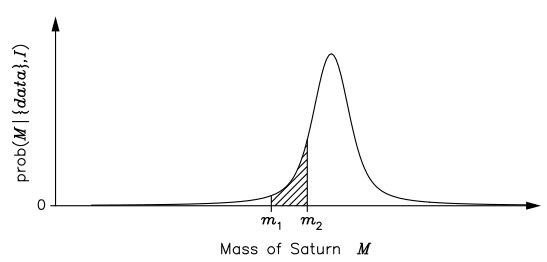
\includegraphics[width=0.9\linewidth]{fig/sivia_fig_1_2.png}}

\vspace{6mm}



% !split

\begin{quote}
To Laplace, the (shaded) area under the posterior pdf curve between $m_1$ and $m_2$ was a measure of how much he believed that the mass of Saturn lay in the range $m_1 \le M \le m_2$. As such, the position of the maximum of the posterior pdf represents a best estimate of the mass; its width, or spread, about this optimal value gives an indication of the uncertainty in the estimate. Laplace stated that: ‘ . . . it is a bet of 11,000 to 1 that the error of this result is not 1/100th of its value.’ He would have won the bet, as another 150 years’ accumulation of data has changed the estimate by only 0.63\%!
\end{quote}


% !split

\begin{quote}
According to the frequency definition, however, we are not permitted to use probability theory to tackle this problem. This is because the mass of Saturn is a constant and not a random variable; therefore, it has no frequency distribution and so probability theory cannot be used.

If the pdf [of Fig.~1.2] had to be interpreted in terms of the frequency definition, we would have to imagine a large ensemble of universes in which everything remains constant apart from the mass of Saturn.
\end{quote}


% !split

\begin{quote}
As this scenario appears quite far-fetched, we might be inclined to think of [Fig.~1.2] in terms of the distribution of the measurements of the mass in many repetitions of the experiment. Although we are at liberty to think about a problem in any way that facilitates its solution, or our understanding of it, having to seek a frequency interpretation for every data analysis problem seems rather perverse.
For example, what do we mean by the ‘measurement of the mass’ when the data consist of orbital periods? Besides, why should we have to think about many repetitions of an experiment that never happened? What we really want to do is to make the best inference of the mass given the (few) data that we actually have; this is precisely the Bayes and Laplace view of probability.
\end{quote}


% !split

\begin{quote}
Faced with the realization that the frequency definition of probability theory did not permit most real-life scientific problems to be addressed, a new subject was invented — statistics! To estimate the mass of Saturn, for example, one has to relate the mass to the data through some function called the statistic; since the data are subject to ‘random’ noise, the statistic becomes the random variable to which the rules of probability the- ory can be applied. But now the question arises: How should we choose the statistic? The frequentist approach does not yield a natural way of doing this and has, therefore, led to the development of several alternative schools of orthodox or conventional statis- tics. The masters, such as Fisher, Neyman and Pearson, provided a variety of different principles, which has merely resulted in a plethora of tests and procedures without any clear underlying rationale. This lack of unifying principles is, perhaps, at the heart of the shortcomings of the cook-book approach to statistics that students are often taught even today.
\end{quote}


% !split
\section{Probability density functions (pdf:s)}

\begin{block_mdfboxadmon}[]

\begin{itemize}
 \item $p(A|B)$ reads “probability of $A$ given $B$”

 \item Simplest examples are discrete, but physicists often interested in continuous case, e.g., parameter estimation.

 \item When integrated, continuous pdfs become probabilities $\Rightarrow$ pdfs are NOT dimensionless, even though probabilities are.

 \item 68\%, 95\%, etc. intervals can then be computed by integration 

 \item Certainty about a parameter corresponds to $p(x) = \delta(x-x_0)$
\end{itemize}

\noindent
\end{block_mdfboxadmon} % title: 



% !split
% ======= pdfs =======
% !split
\subsection{Properties of PDFs}

\begin{block_mdfboxadmon}[]

There are two properties that all PDFs must satisfy. The first one is
positivity (assuming that the PDF is normalized)

\begin{equation*}
0 \leq p(x).
\end{equation*}
Naturally, it would be nonsensical for any of the values of the domain
to occur with a probability less than $0$. Also,
the PDF must be normalized. That is, all the probabilities must add up
to unity.  The probability of ``anything'' to happen is always unity. For
discrete and continuous PDFs, respectively, this condition is
\begin{align*}
\sum_{x_i\in\mathbb D} p(x_i) & =  1,\\
\int_{x\in\mathbb D} p(x)\,dx & =  1.
\end{align*}
\end{block_mdfboxadmon} % title: 



% !split
\subsection{Important distributions, the uniform distribution}

\begin{block_mdfboxadmon}[]
Let us consider some important, univariate distributions.
The first one
is the most basic PDF; namely the uniform distribution
\begin{equation}
p(x) = \frac{1}{b-a}\theta(x-a)\theta(b-x).
\label{eq:unifromPDF}
\end{equation}
For $a=0$ and $b=1$ we have 
\[
p(x) = \left\{
\begin{array}{ll}
1 & x \in [0,1],\\
0 & \mathrm{otherwise}
\end{array}
\right.
\]
\end{block_mdfboxadmon} % title: 



% !split
\subsection{Gaussian distribution}

\begin{block_mdfboxadmon}[]
The second one is the univariate Gaussian Distribution
\begin{equation*}
p(x) = \frac{1}{\sigma\sqrt{2\pi}} \exp{(-\frac{(x-\mu)^2}{2\sigma^2})},
\end{equation*}
with mean value $\mu$ and standard deviation $\sigma$. If $\mu=0$ and $\sigma=1$, it is normally called the \textbf{standard normal distribution}
\begin{equation*}
p(x) = \frac{1}{\sqrt{2\pi}} \exp{(-\frac{x^2}{2})},
\end{equation*}
\end{block_mdfboxadmon} % title: 




% !split
\subsection{Expectation values}

\begin{block_mdfboxadmon}[]
Let $h(x)$ be an arbitrary continuous function on the domain of the stochastic
variable $X$ whose PDF is $p(x)$. We define the \emph{expectation value}
of $h$ with respect to $p$ as follows

\begin{equation}
\langle h \rangle_X \equiv \int\! h(x)p(x)\,dx
\label{eq:expectation_value_of_h_wrt_p}
\end{equation}
Whenever the PDF is known implicitly, like in this case, we will drop
the index $X$ for clarity.  
A particularly useful class of special expectation values are the
\emph{moments}. The $n$-th moment of the PDF $p$ is defined as
follows
\begin{equation*}
\langle x^n \rangle \equiv \int\! x^n p(x)\,dx
\end{equation*}
\end{block_mdfboxadmon} % title: 



% !split
\subsection{Stochastic variables and the main concepts, mean values}

\begin{block_mdfboxadmon}[]
The zero-th moment $\langle 1\rangle$ is just the normalization condition of
$p$. The first moment, $\langle x\rangle$, is called the \emph{mean} of $p$
and often denoted by the letter $\mu$
\begin{equation*}
\langle x\rangle  \equiv \mu = \int x p(x)dx,
\end{equation*}
for a continuous distribution and 
\begin{equation*}
\langle x\rangle  \equiv \mu = \sum_{i=1}^N x_i p(x_i),
\end{equation*}
for a discrete distribution. 
Qualitatively it represents the centroid or the average value of the
PDF and is therefore simply called the expectation value of $p(x)$.
\end{block_mdfboxadmon} % title: 



% !split
\subsection{Mean, median, average}

\begin{block_mdfboxadmon}[]
The values of the \textbf{mode}, \textbf{mean}, \textbf{median} can all be used as point estimates for the "probable" value of $x$. For some pdfs, they will all be the same.
\end{block_mdfboxadmon} % title: 




\begin{figure}[!ht]  % 
  \centerline{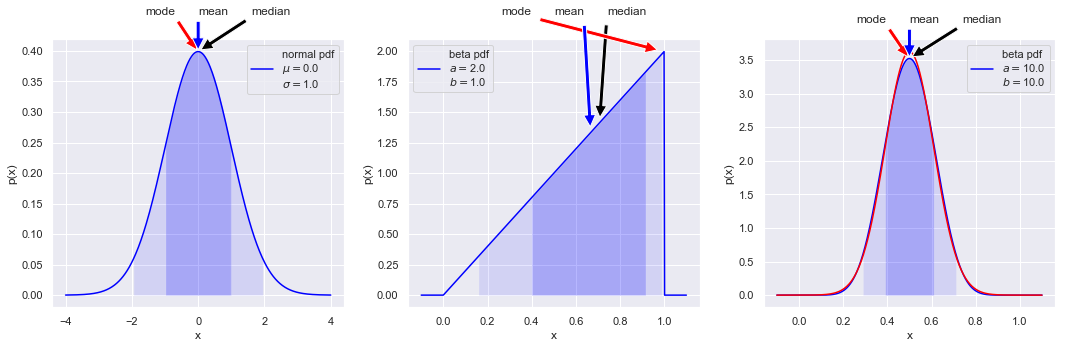
\includegraphics[width=1.0\linewidth]{fig/pdfs.png}}
  \caption{
  The 68\%/95% probability regions are shown in dark/light shading. When applied to Bayesian posteriors, these are known as credible intervals or DoBs (degree of belief intervals) or Bayesian confidence intervals. The horizontal extent on the $x$-axis translates into the vertical extent of the error bar or error band for $x$.
  }
\end{figure}
%\clearpage % flush figures 


% !split
\subsection{Stochastic variables and the main concepts, central moments, the variance}

\begin{block_mdfboxadmon}[]

A special version of the moments is the set of \emph{central moments}, the n-th central moment defined as
\begin{equation*}
\langle (x-\langle x\rangle )^n\rangle  \equiv \int\! (x-\langle x\rangle)^n p(x)\,dx
\end{equation*}
The zero-th and first central moments are both trivial, equal $1$ and
$0$, respectively. But the second central moment, known as the
\emph{variance} of $p$, is of particular interest. For the stochastic
variable $X$, the variance is denoted as $\sigma^2_X$ or $\mathrm{Var}(X)$
\begin{align*}
\sigma^2_X &=\mathrm{Var}(X) =  \langle (x-\langle x\rangle)^2\rangle  =
\int (x-\langle x\rangle)^2 p(x)dx\\
& =  \int\left(x^2 - 2 x \langle x\rangle^{2} +\langle x\rangle^2\right)p(x)dx\\
& =  \langle x^2\rangle - 2 \langle x\rangle\langle x\rangle + \langle x\rangle^2\\
& =  \langle x^2 \rangle - \langle x\rangle^2
\end{align*}
The square root of the variance, $\sigma =\sqrt{\langle (x-\langle x\rangle)^2\rangle}$ is called the 
\textbf{standard deviation} of $p$. It is the RMS (root-mean-square)
value of the deviation of the PDF from its mean value, interpreted
qualitatively as the ``spread'' of $p$ around its mean.
\end{block_mdfboxadmon} % title: 





% !split
\subsection{Probability Distribution Functions}

\begin{block_mdfboxadmon}[]

The following table collects properties of probability distribution functions.
In our notation we reserve the label $p(x)$ for the probability of a certain event,
while $P(x)$ is the cumulative probability. 




\begin{tabular}{lcc}
\hline
\multicolumn{1}{c}{  } & \multicolumn{1}{c}{ Discrete PDF } & \multicolumn{1}{c}{ Continuous PDF } \\
\hline
Domain        & $\left\{x_1, x_2, x_3, \dots, x_N\right\}$ & $[a,b]$                              \\
Probability   & $p(x_i)$                                   & $p(x)dx$                             \\
Cumulative    & $P_i=\sum_{l=1}^ip(x_l)$                   & $P(x)=\int_a^xp(t)dt$                \\
Positivity    & $0 \le p(x_i) \le 1$                       & $p(x) \ge 0$                         \\
Positivity    & $0 \le P_i \le 1$                          & $0 \le P(x) \le 1$                   \\
Monotonic     & $P_i \ge P_j$ if $x_i \ge x_j$             & $P(x_i) \ge P(x_j)$ if $x_i \ge x_j$ \\
Normalization & $P_N=1$                                    & $P(b)=1$                             \\
\hline
\end{tabular}


\noindent
\end{block_mdfboxadmon} % title: 




% !split
\subsection{Quick introduction to  \texttt{scipy.stats} }
If you google \texttt{scipy.stats}, you'll likely get the manual page as the first hit: \href{{https://docs.scipy.org/doc/scipy/reference/stats.html}}{https://docs.scipy.org/doc/scipy/reference/stats.html}. Here you'll find a long list of the continuous and discrete distributions that are available, followed (scroll way down) by many different methods (functions) to extract properties of a distribution (called Summary Statistics) and do many other statistical tasks.

Follow the link for any of the distributions (your choice!) to find its mathematical definition, some examples of how to use it, and a list of methods. Some methods of interest to us here:

\begin{itemize}
 \item \texttt{mean()} - Mean of the distribution.

 \item \texttt{median()} - Median of the distribution.

 \item \texttt{pdf(x)} - Value of the probability density function at x.

 \item \texttt{rvs(size=numpts)} - generate numpts random values of the pdf.

 \item \texttt{interval(alpha)} - Endpoints of the range that contains alpha percent of the distribution.
\end{itemize}

\noindent
% !split
\section{The Bayesian recipe}

\begin{block_mdfboxadmon}[]
Assess hypotheses by calculating their probabilities $p(H_i | \ldots)$ conditional on known and/or presumed information using the rules of probability theory.
\end{block_mdfboxadmon} % title: 




\begin{block_mdfboxadmon}[]
Probability Theory Axioms:
\begin{description}
\item[Product (AND) rule :] 
  $p(A, B | I) = p(A|I) p(B|A, I) = p(B|I)p(A|B,I)$\\
  Should read $p(A,B|I)$ as the probability for propositions $A$ AND $B$ being true given that $I$ is true.

\item[Sum (OR) rule:] 
  $p(A + B | I) = p(A | I) + p(B | I) - p(A, B | I)$\\
  $p(A+B|I)$ is the probability that proposition $A$ OR $B$ is true given that $I$ is true.

\item[Normalization:] 
  $p(A|I) + p(\bar{A}|I) = 1$\\
  $\bar{A}$ denotes the proposition that $A$ is false.
\end{description}

\noindent
\end{block_mdfboxadmon} % title: 



% !split
\subsection{Bayes' theorem}

\begin{block_mdfboxadmon}[]
Bayes' theorem follows directly from the product rule

\[
p(A|B,I) = \frac{p(B|A,I) p(A|I)}{p(B|I)}.
\]

The importance of this property to data analysis becomes apparent if we replace $A$ and $B$ by hypothesis($H$) and data($D$):
\begin{align}
p(H|D,I) &= \frac{p(D|H,I) p(H|I)}{p(D|I)}.
\label{eq:bayes}
\end{align}
The power of Bayes’ theorem lies in the fact that it relates the quantity of interest, the probability that the hypothesis is true given the data, to the term we have a better chance of being able to assign, the probability that we would have observed the measured data if the hypothesis was true.
\end{block_mdfboxadmon} % title: 



% !split

\begin{block_mdfboxadmon}[]
The various terms in Bayes’ theorem have formal names. 
\begin{itemize}
\item The quantity on the far right, $p(H|I)$, is called the \emph{prior} probability; it represents our state of knowledge (or ignorance) about the truth of the hypothesis before we have analysed the current data. 

\item This is modified by the experimental measurements through $p(D|H,I)$, the \emph{likelihood} function, 

\item The denominator $p(D|I)$ is called the \emph{evidence}. It does not depend on the hypothesis and can be regarded as a normalization constant.

\item Together, these yield the \emph{posterior} probability, $p(H|D, I )$, representing our state of knowledge about the truth of the hypothesis in the light of the data. 
\end{itemize}

\noindent
In a sense, Bayes’ theorem encapsulates the process of learning.
\end{block_mdfboxadmon} % title: 



% !split
\subsection{The friends of Bayes' theorem}

\begin{block_mdfboxadmon}[]
\begin{description}
\item[Normalization:] 
  $\sum_i p(H_i|I) = 1$.

\item[Marginalization:] 
  $p(A|I) = \sum_i p(H_i|A,I) p(A|I) = \sum_i p(A,H_i|I)$.
\end{description}

\noindent
In the above, $H_i$ is an exclusive and exhaustive list of hypotheses. For example,let’s imagine that there are five candidates in a presidential election; then $H_1$ could be the proposition that the first candidate will win, and so on. The probability that $A$ is true, for example that unemployment will be lower in a year’s time (given all relevant information $I$, but irrespective of whoever becomes president) is given by $\sum_i p(A,H_i|I)$ as shown by using normalization and applying the product rule.
\end{block_mdfboxadmon} % title: 



% !split

\begin{block_mdfboxadmon}[]
\begin{description}
\item[Normalization (continuum limit):] 
  $\int dx p(x|I) = 1$.

\item[Marginalization (continuum limit):] 
  $p(y|I) = \int dx p(x,y|I)$.
\end{description}

\noindent
In the continuum limit of propositions we must understand $p(\ldots)$ as a pdf (probability density function).

Marginalization is a very powerful device in data analysis because it enables us to deal with nuisance parameters; that is, quantities which necessarily enter the analysis but are of no intrinsic interest. The unwanted background signal present in many experimental measurements are examples of nuisance parameters.
\end{block_mdfboxadmon} % title: 



% !split
\section{Example: Is this a fair coin?}
Let us begin with the analysis of data from a simple coin-tossing experiment. 
Given that we had observed 6 heads in 8 flips, would you think it was a fair coin? By fair, we mean that we would be prepared to lay an even 1 : 1 bet on the outcome of a flip being a head or a tail. If we decide that the coin was fair, the question which follows naturally is how sure are we that this was so; if it was not fair, how unfair do we think it was? Furthermore, if we were to continue collecting data for this particular coin, observing the outcomes of additional flips, how would we update our belief on the fairness of the coin?

% !split
A sensible way of formulating this problem is to consider a large number of hypotheses about the range in which the bias-weighting of the coin might lie. If we denote the bias-weighting by $p_H$, then $p_H = 0$ and $p_H = 1$ can represent a coin which produces a tail or a head on every flip, respectively. There is a continuum of possibilities for the value of $p_H$ between these limits, with $p_H = 0.5$ indicating a fair coin. Our state of knowledge about the fairness, or the degree of unfairness, of the coin is then completely summarized by specifying how much we believe these various propositions to be true. 

% !split
Let us perform a computer simulation of a coin-tossing experiment. This provides the data that we will be analysing.

\begin{lstlisting}[language=Python,style=blue1]
import numpy as np
import matplotlib.pyplot as plt
\end{lstlisting}

\begin{lstlisting}[language=Python,style=blue1]
np.random.seed(999)         # for reproducibility
pH=0.6                       # biased coin
flips=np.random.rand(2**12) # simulates 4096 coin flips
heads=flips<pH              # boolean array, heads[i]=True if flip i is heads
\end{lstlisting}

% !split
In the light of this data, our inference about the fairness of this coin is summarized by the conditional pdf: $p(p_H|D,I)$. This is, of course, shorthand for the limiting case of a continuum of propositions for the value of $p_H$; that is to say, the probability that $p_H$ lies in an infinitesimally narrow range is given by $p(p_H|D,I) dp_H$. 

% !split
To estimate this posterior pdf, we need to use Bayes’ theorem (\ref{eq:bayes}). We will ignore the denominator $p(D|I)$ as it does not involve bias-weighting explicitly, and it will therefore not affect the shape of the desired pdf. At the end we can evaluate the missing constant subsequently from the normalization condition 
\begin{equation}
\int_0^1 p(p_H|D,I) dp_H = 1.
\label{eq:coin_posterior_norm}
\end{equation}

% !split
The prior pdf, $p(p_H|I)$, represents what we know about the coin given only the information $I$ that we are dealing with a ‘strange coin’. We could keep a very open mind about the nature of the coin; a simple probability assignment which reflects this is a uniform, or flat, prior
\begin{equation}
p(p_H|I) = \left\{ \begin{array}{ll}
1 & 0 \le p_H \le 1, \\
0 & \mathrm{otherwise}.
\end{array} \right.
\label{eq:coin_prior_uniform}
\end{equation}
We will get back later to the choice of prior and its effect on the analysis.

% !split
This prior state of knowledge, or ignorance, is modified by the data through the likelihood function $p(D|p_H,I)$. It is a measure of the chance that we would have obtained the data that we actually observed, if the value of the bias-weighting was given (as known). If, in the conditioning information $I$, we assume that the flips of the coin were independent events, so that the outcome of one did not influence that of another, then the probability of obtaining the data `H heads in N tosses' is given by the binomial distribution (we leave a formal definition of this to a statistics textbook)
\begin{equation}
p(D|p_H,I) \propto p_H^H (1-p_H)^{N-H}.
\end{equation}

% !split
It seems reasonable because $p_H$ is the chance of obtaining a head on any flip, and there were $H$ of them, and $1-p_H$ is the corresponding probability for a tail, of which there were $N-H$. We note that this binomial distribution also contains a normalization factor, but we will ignore it since it does not depend explicitly on $p_H$, the quantity of interest. It will be absorbed by the normalization condition (\ref{eq:coin_posterior_norm}).

% !split
We perform the setup of this Bayesian framework on the computer.

\begin{lstlisting}[language=Python,style=blue1]
def prior(pH):
    p=np.zeros_like(pH)
    p[(0<=pH)&(pH<=1)]=1      # allowed range: 0<=pH<=1
    return p                # uniform prior
def likelihood(pH,data):
    N = len(data)
    no_of_heads = sum(data)
    no_of_tails = N - no_of_heads
    return pH**no_of_heads * (1-pH)**no_of_tails
def posterior(pH,data):
    p=prior(pH)*likelihood(pH,data)
    norm=np.trapz(p,pH)
    return p/norm
\end{lstlisting}

% !split
The next step is to confront this setup with the simulated data. To get a feel for the result, it is instructive to see how the posterior pdf evolves as we obtain more and more data pertaining to the coin. The results of such an analyses is shown in Fig.~\ref{fig:coinflipping}. 

\begin{lstlisting}[language=Python,style=blue1]
pH=np.linspace(0,1,1000)
fig, axs = plt.subplots(nrows=4,ncols=3,sharex=True,sharey='row',figsize=(14,14))
axs_vec=np.reshape(axs,-1)
axs_vec[0].plot(pH,prior(pH))
for ndouble in range(11):
    ax=axs_vec[1+ndouble]
    ax.plot(pH,posterior(pH,heads[:2**ndouble]))
    ax.text(0.1, 0.8, '$N={0}$'.format(2**ndouble), transform=ax.transAxes)
for row in range(4): axs[row,0].set_ylabel('$p(p_H|D_\mathrm{obs},I)$')
for col in range(3): axs[-1,col].set_xlabel('$p_H$')
\end{lstlisting}

% !split

\begin{figure}[!ht]  % fig:coinflipping
  \centerline{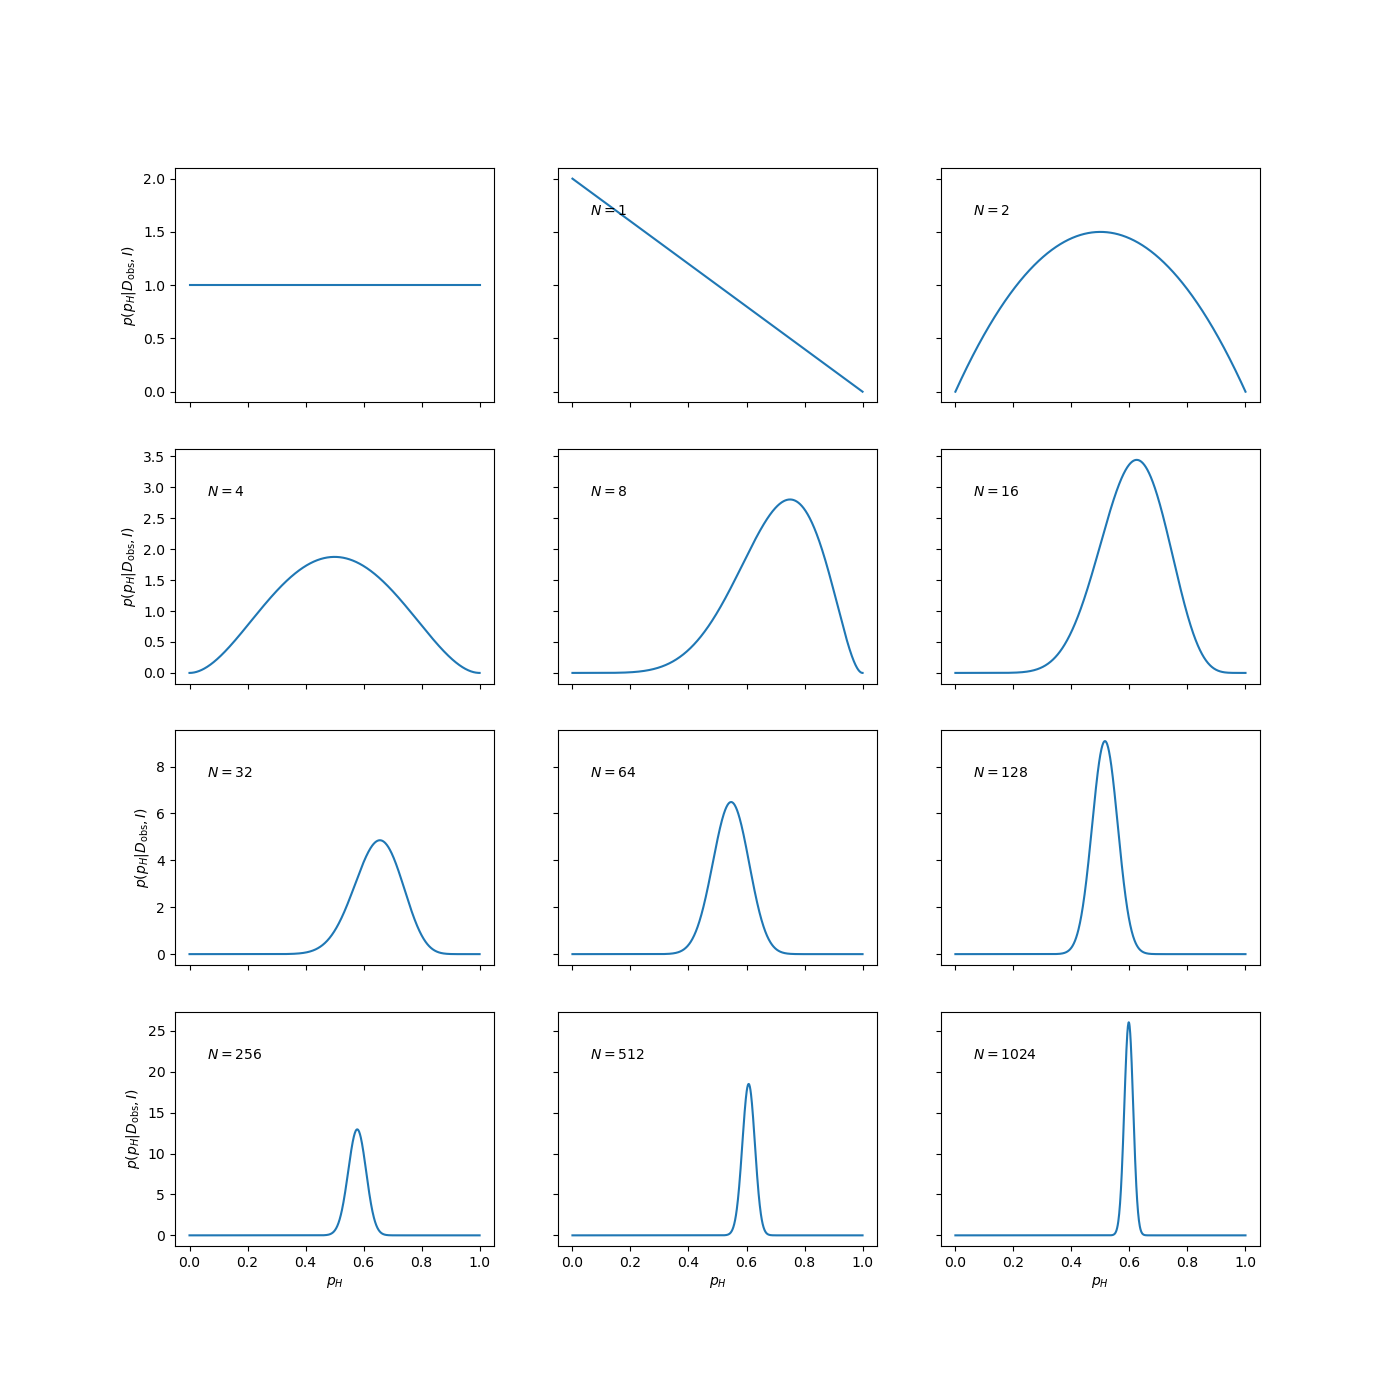
\includegraphics[width=0.95\linewidth]{fig/coinflipping_fig_1.png}}
  \caption{
  The evolution of the posterior pdf for the bias-weighting of a coin, as the number of data available increases. The figure on the top left-hand corner of each panel shows the number of data included in the analysis. \label{fig:coinflipping}
  }
\end{figure}
%\clearpage % flush figures fig:coinflipping


% !split
The panel in the top left-hand corner shows the posterior pdf for $p_H$ given no data, i.e., it is the same as the prior pdf of Eq. (\ref{eq:coin_prior_uniform}). It indicates that we have no more reason to believe that the coin is fair than we have to think that it is double-headed, double-tailed, or of any other intermediate bias-weighting.

% !split
The first flip is obviously tails. At this point we have no evidence that the coin has a side with heads, as indicated by the pdf going to zero as $p_H \to 1$. The second flip is obviously heads and we have now excluded both extreme options $p_H=0$ (double-tailed) and $p_H=1$ (double-headed). We can note that the posterior at this point has the simple form $p(p_H|D,I) = p_H(1-p_H)$ for $0 \le p_H \le 1$.

% !split
The remainder of Fig.~\ref{fig:coinflipping} shows how the posterior pdf evolves as the number of data analysed becomes larger and larger. We see that the position of the maximum moves around, but that the amount by which it does so decreases with the increasing number of observations. The width of the posterior pdf also becomes narrower with more data, indicating that we are becoming increasingly confident in our estimate of the bias-weighting. For the coin in this example, the best estimate of $p_H$ eventually converges to 0.6, which, of course, was the value chosen to simulate the flips.

% !split
\section{Take aways: Coin tossing}

% !bpop
\begin{itemize}
\item The Bayesian posterior $p(p_H | D, I)$ is proportional to the product of the prior and the likelihood (which is given by a binomial distribution in this case).

\item We can do this analysis sequentially (updating the prior after each toss and then adding new data; but don't use the same data more than once!). Or we can analyze all data at once. 

\item Why (and when) are these two approaches equivalent, and why should we not use the same data more than once?
\end{itemize}

\noindent
% !epop

% !split
% !bpop
\begin{itemize}
\item Possible point estimates for the value of $p_H$ could be the maximum (mode), mean, or median of this posterior pdf. 

\item Bayesian p% degree-of-belief (DoB) intervals correspond to ranges in which we would give a p% odds of finding the true value for $p_H$ based on the data and the information that we have.

\item The frequentist point estimate is $p_H^* = \frac{H}{N}$. It actually corresponds to one of the point estimates from the Bayesian analysis for a specific prior? Which point estimate and which prior?
\end{itemize}

\noindent
% !epop

% ------------------- end of main content ---------------

% #ifdef PREAMBLE
\end{document}
% #endif

